\documentclass[12pt]{article}
\usepackage{amsmath}
\usepackage{array}
% \usepackage{gensymb}
\usepackage{geometry}
\usepackage{graphicx}
\usepackage{pgfplots}
\usepackage{siunitx}
\usepackage{wrapfig}

\title{Homework \#11}
\author{Donald Aingworth IV}
\date{November 6, 2024}

\pgfplotsset{width=8cm,compat=1.9}
\usepgfplotslibrary{external}
% \tikzexternalize

\begin{document}

\DeclareSIUnit{\mile}{mi}
\DeclareSIUnit{\gal}{gal}
\DeclareSIUnit{\foot}{ft}
\DeclareSIUnit{\h}{h}

\maketitle

\pagebreak
\section*{Problem 1}
A neutron at rest decays into a proton, an electron, and a neutrino. If the proton's momentum is $3.00\times10^{-24}$ kg m/s in the direction 37\unit{\degree} N of E and the electron's momentum is $4.00\times10^{-24}$ kg m/s in the direction 53\unit{\degree} S of W, what is the momentum of the neutrino?

\subsection*{Solution}


\pagebreak
\section*{Problem 2}
\begin{wrapfigure}{r}{0.35\textwidth}
    \vspace{-30pt}
    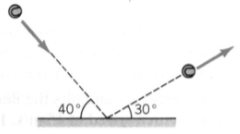
\includegraphics[width=0.35\textwidth]{graph_2.png} 
    % \label{fig:wrapfig}
\end{wrapfigure}
A 60.0-g tennis ball strikes the ground at 25.0 m/s at 40\unit{\degree} to the horizontal. It bounces off at 20.0 m/s at 30\unit{\degree} to the horizontal. (a) Find the impulse exerted on the ball. (b) If the collision lasted 5.00 ms, find the average force exerted on the ball by the court.

\subsection*{Solution}


\pagebreak
\section*{Problem 3}
A 1000-kg Subaru at rest at a stoplight is struck from the rear by a 1400-kg Pontiac. They couple together and leave skid marks 4.25 m long. The coefficient of kinetic friction is 0.6. (a) What was their common speed just after the collision? (b) What was the speed of the Pontiac just prior to the collision?

\subsection*{Solution}


\pagebreak
\section*{Problem 4}
Two particles with masses $m_1$ and $m_2$ travel toward each other with velocities $v_{1,i}$ and $v_{2,i}$. They collide and stick together. Show that the loss in kinetic energy is
\[ \frac{m_1 m_2 \left(v_{1,i} - v_{2,i}\right)^2}{2(m_1 + m_2)} \]

\subsection*{Solution}


\pagebreak
\section*{Problem 5}
\begin{wrapfigure}{r}{0.35\textwidth}
    \vspace{-30pt}
    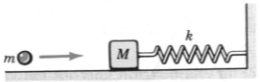
\includegraphics[width=0.35\textwidth]{graph_5.png} 
    % \label{fig:wrapfig}
\end{wrapfigure}
A projectile of mass 0.25 kg moving at 24.0 m/s collides with and sticks to a 1.75-kg block that is connected to a spring for which k = 40.0 N/m, as in the figure below. The block is initially on a frictionless part of a horizontal surface but starts to slide on a rough section immediately after the collision. If the maximum compression of the spring is 0.5 m, what is the force of friction on the block?

\subsection*{Solution}


\pagebreak
\section*{Problem 6}
\begin{wrapfigure}{r}{0.35\textwidth}
    \vspace{-58pt}
    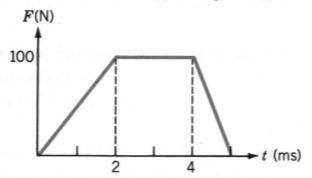
\includegraphics[width=0.35\textwidth]{graph_6.png} 
    % \label{fig:wrapfig}
\end{wrapfigure}
From the F versus t curve shown to the right, find: (a) the impulse; (b) the average force.

\subsection*{Solution}


\pagebreak
\section*{Problem 7}
A nucleus of radioactive radium ($^{226}$Ra), initially at rest, decays into a radon nucleus ($^{222}$Rn) and an $\alpha$-particle (a $^{4}$He nucleus). If the kinetic energy of the $\alpha$-particle is $6.72 \times 10^{-13}$ J, what is (a) the recoil speed of the radon nucleus, and (b) its kinetic energy? The superscripts indicate, roughly, the mass of each nucleus in unified mass units (u), where 1 u = $1.66 \times 10^{-27}$ kg.

\subsection*{Solution}


\pagebreak
\section*{Problem 8}
\begin{wrapfigure}{r}{0.35\textwidth}
    \vspace{-30pt}
    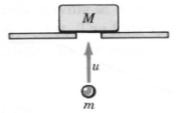
\includegraphics[width=0.35\textwidth]{graph_8.png} 
    % \label{fig:wrapfig}
\end{wrapfigure}
A projectile of mass $m$ = 200 g strikes a stationary block of mass $M$ = 1.30 kg from below with speed $u$ = 30.0 m/s as shown in the figure below. The projectile embeds in the block. (a) To what height does the block rise? (b) What is the loss in kinetic energy due to the collision?

\subsection*{Solution}

\end{document}